%%%%%%%%%%%%%%%%%%%%%%%%%%%%%%%%%%%%%% 
\section[Path Planning Simulation]{Path Planning Simulation}
%%%%%%%%%%%%%%%%%%%%%%%%%%%%%  

\newcommand{\revised}[1]{{\color{red}#1}}

\subsection{Modelling}
\label{subsec:modelling}
The data on the distribution of mosquitoes is given for a two-dimensional grid environment; the grid size
is induced by the size of the screen, the available data and the desired resolution of the extracted map. 
For each pixel $p_i\in P$, we are given a relative value
$c(p_i)$ that describes the estimated a-priori density of mosquitoes, based on data obtained from boustrophedon (back and forth) scans of the area by the UAV;
this implies that only a subset of pixels carry a significant value.
Visiting one of the pixels corresponds to sampling and mapping the actual density distribution of mosquitoes. 
For a dense distribution of mosquitoes
(which is the case for the instances relevant for pest control), multiple visits to the same pixel do not contribute additional
knowledge. As a consequence, the objective is to maximize the sampling value of the set $S\subseteq P$ of visited pixels, 
i.e., $\max_{S\subseteq P} \sum_{p_i\in S} c(p_i)$ {within the available battery capacity}; this may be over the course of a single closed trajectory, or over
a combination of multiple roundtrips. 

Planning good trajectories for a UAV is not subject to the same curvature constraints of an ordinary aircraft
because UAVs can turn on the spot. However, turns are a critical aspect of path
planning due to their impact on energy consumption.  Battery capacity is {\em the} limiting factor for  UAV flight time. As shown in Fig.~\ref{fig:turncost}, 
the power output for a desired trajectory is non-uniform.  Flying along a straight path
is relatively inexpensive but turning is energy intensive. 

\begin{figure}[h]
\begin{center}
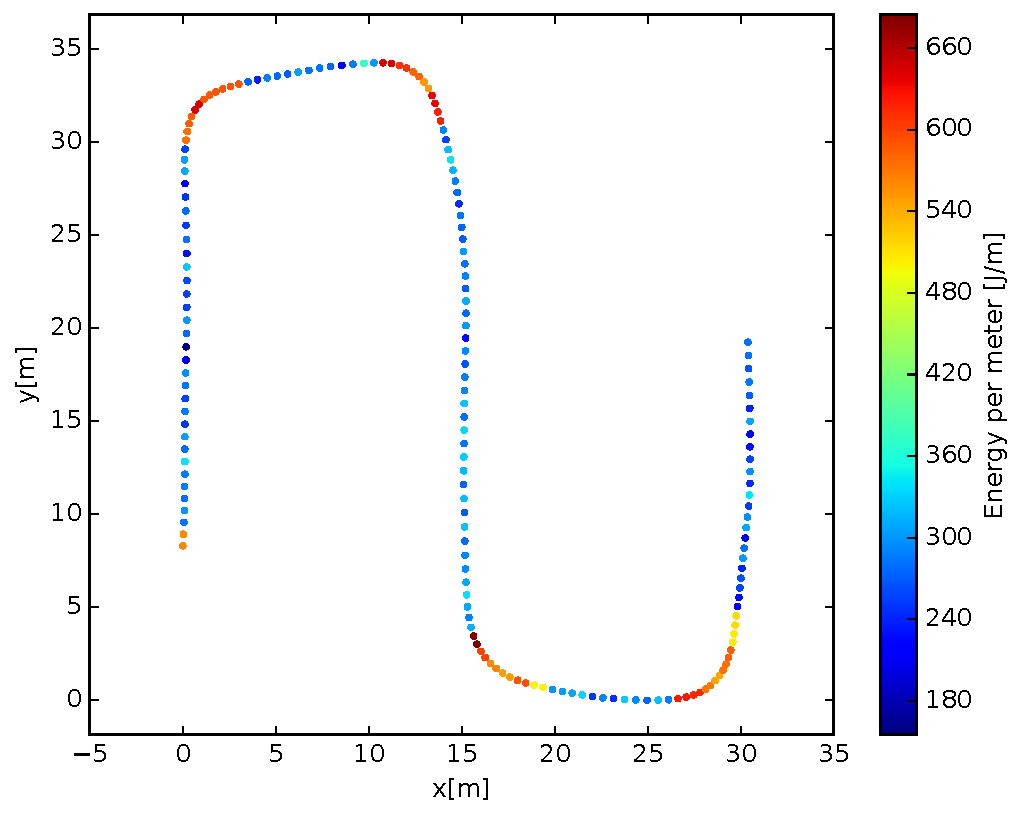
\includegraphics[width=.75\columnwidth]{icra2018/turncost}
\caption[Mosquito hunting drone]{Turns are expensive. See our related video at
\url{https://youtu.be/SFyOMDgdNao} for details, and
\cite{becker2017zapping} for an accompanying abstract.} \label{fig:turncost}
\end{center}
\vspace{-1em}
\end{figure}


As a consequence, we must consider the total turn costs associated
with changing direction, as measured by the turn angle.
As we are not limited by trajectory curvature, we refer to straight-line connections and a finite set of $2\omega$ different
headings for visiting vertices. For the most natural case of orthogonal grids $\omega=2$. When
surveying non-isolated mosquito hotspots (whose size greatly exceeds the size of the UAV), we are not dealing with
isolated pixels and the modeling error of this restriction is small.

%TODO: I guess one can save space here by e.g. skipping subset cover.
Now we consider different trajectory types.
A {\em cycle} is a roundtrip of a subset $S\subseteq P$ that visits all points in $S$ and returns to the origin, a {\em cycle cover} of $P$ is a set of cycles
that together visit all points in $P$, and a {\em tour} is a single cycle that visits all points in $P$. A {\em subset cycle cover} for $S\subset P$ is a cycle
cover that covers at least the points in $S$, while a {\em subset tour} is a tour of at least the points in $S$. For any of these structures, we are interested in
%cycle covers or tours of {\em minimum total turn cost}. 
{cycle covers or tours of {\em minimum total travel cost}. 
The travel/battery cost is a linear combination of the number of pixel transitions (distance) and the weighted number of turns, 
corresponding to the total turn angle.
}
In addition, a {\em minimum turn-cost penalty cycle cover}  or a {\em minimum turn-cost penalty tour}
visits a subset $R\subset P$, such that the sum of total travel cost and the sum $\sum_{i\not\in R} c(p_i)$ of values of 
unvisited pixels is minimized. 
%The travel/battery cost is a linear combination of the number of pixel transitions (distance) and the weighted number of turns, 
%corresponding to the total turn angle.
%Note that the travel cost
%may be a linear combination of turn and travel cost, as long as triangle inequality is satisfied.

\subsection{Computational Complexity}
\label{subsec:complexity}
Finding optimal covering paths that map a given region is closely related to the famous 
\emph{Traveling Salesman Problem (TSP)}, which asks to minimize
total length of a single tour that covers all of a given set of locations. The TSP is one of 
the classic NP-hard problems, so we cannot expect a general method that finds
a provably optimal solution for any  instance in polynomially bounded time.
A generalization of the TSP is
the \emph{Lawnmower Problem} (see Arkin et al.~\cite{arkin2000approximation}, which considers coverage by
a tool of nontrivial size. For the objective of minimizing the total cost (in particular, the turn
cost), Arkin et al.~\cite{arkin2005optimal} showed that finding minimum-turn tours in grid graphs is NP-hard,
even if a minimum-turn cycle cover is given. The complexity of finding a set of multiple cycles that cover a 
given set of locations at minimum total turn cost had remained elusive for many years; \emph{Problem~{53}} in \emph{The Open Problems Project}
%edited by Demaine, Mitchell, and O'Rourke~\cite{openproblemproject}
asks for the complexity of finding a minimum-cost (full) cycle cover in a 2-dimensional grid graph. This is not 
obvious: large parts of a solution can usually easily be deduced by local information and 2-factor techniques.
Arkin et al. showed~\cite{arkin2005optimal,arkin2001optimal} that the full coverage variant in {\em thin} grid graphs (which do not contain a $2\times 2$ square,
so every pixel is a boundary pixel) is solvable in polynomial time. In separate work~\cite{dom3}, two of us were able to resolve this
issue by showing that finding a cycle cover of minimum turn cost is  NP-hard.

\subsection{Mathematical Optimization}
\label{subsec:complexity}
A powerful approach for finding optimal solutions to instances of NP-hard problems is the use
of Integer Programming (IP). While solving an IP still requires exponential time in the worst case,
using carefully crafted mathematical models in combination with specific algorithm engineering and available
IP solvers enables solving instances of considerable size to provable optimality.
For our purposes, we can describe the problem as follows. 

\paragraph{Penalty Cycle Covers}
The set $P$ of pixels corresponds to a given grid graph $G(P,E)$ in which each pixel $p_j\in P$ is adjacent to the set $N(p_j)$
of pixels in $P$ that share an edge with $p_j$.
Each vertex $p_j\in P$ has a scalar reward $c(p_j)$ for visiting (or penalty for not visiting), 
and a function $\text{cost}_j(i,k)\in \mathbb{Z}^+_0$  that maps the cost of traveling from $p_i$ to $p_j$ to $p_k$, where  $p_i,p_k\in N(p_j)$ are adjacent pixels to   $p_j$.
This cost is symmetric, i.e. $\text{cost}_j(i,k)=\text{cost}_j(k,i)$. %TODO: Or cost(ijk) or cost(i,j,k) or cost(p_i, p_j, p_k)
The integer program uses two types of variables: integer variables
$x_{ijk}=x_{kji}$ that state how often passage $p_i-p_j-p_k$ or $p_k-p_j-p_i$ is used and
Boolean variables $y_{j}$ that indicate that the pixel $p_j\in V$ is not covered,
i.e., the penalty is paid.  This results in the following formulation: 
%IP Formulation TODO
%\begin{strip}
%\begin{eqnarray}
%	\min & \displaystyle  \sum_{p_j\in P} \sum_{p_i,p_k\in N(p_j)} \text{cost}_j(i,k) \cdot x_{ijk} + \sum_{p_j\in P}c(p_j) \cdot y_j\label{eq:obj}\\
%	\text{s.t.}			& 1\leq\displaystyle 4 \cdot y_j +\sum_{p_i,p_k\in N(p_j)} x_{ijk} \leq 4&\forall p_j\in P \label{eq:ip:constr1}\\
%						& \displaystyle 2 \cdot x_{jij} +\sum_{p_k\in N(p_i), p_k\not= p_j}x_{jik} = 2 \cdot x_{iji}+\sum_{p_k\in N(p_j), p_k\not= p_i}x_{ijk}  & \forall \{p_i,p_j\}\in E \label{eq:ip:constr2}\\
%						& x_{ijk}\in\mathbb{N}_0, y_j\in \mathbb{B} & \forall p_j\in P, \{p_i,p_k\}\subseteq N(p_j)
%\end{eqnarray}
%\end{strip}
\begin{eqnarray}
	\min  \displaystyle  \sum_{p_j\in P} \sum_{p_i,p_k\in N(p_j)} \text{cost}_j(i,k) \cdot x_{ijk} + \sum_{p_j\in P}c(p_j) \cdot y_j\label{eq:obj}
\end{eqnarray}
with constraints
\begin{eqnarray}
	 1\leq\displaystyle 4 \cdot y_j +\sum_{p_i,p_k\in N(p_j)} x_{ijk} \leq 4, &\forall p_j\in P \label{eq:ip:constr1}
\end{eqnarray}
\begin{eqnarray}	
%	\displaystyle  x_{jij}   \underset{ p_k\in N(p_i), p_k\not = p_j}{+ \tfrac{1}{2}\sum x_{jik}}  \!\!    =   x_{iji}      \underset{p_k\in N(p_j), p_k\not= p_i}{+ \tfrac{1}{2}\sum x_{ijk}},  & \forall \{p_i,p_j\}\in E 
	\displaystyle 2 x_{jij}  \!\!\!   \underset{ p_k\in N(p_i), p_k\not = p_j}{+\sum x_{jik}}  \!\!\!\!\!    = 2  x_{iji} \!\!\!     \underset{p_k\in N(p_j), p_k\not= p_i}{+\sum x_{ijk}},  & \forall \{p_i,p_j\}\in E \label{eq:ip:constr2}
\end{eqnarray}
\begin{eqnarray}	
	 x_{ijk}\in\mathbb{N}_0, y_j\in \mathbb{B} ,& \forall p_j\in P, \{p_i,p_k\}\subseteq N(p_j)  \label{eq:ip:constrINTS}
\end{eqnarray}


%Describe IP
The objective function in Eq.~\ref{eq:obj} minimizes the total cost of the cycles and the uncovered pixels.
Eq.~\ref{eq:ip:constr1} enforces a pixel to be covered or the \emph{not covered} variable to be set to {\tt true}.
Arkin et al.~\cite{arkin2005optimal} showed that no pixel needs to be visited more than four times, otherwise a simple local optimization 
can be performed.
Eq.~\ref{eq:ip:constr2} enforces the transitions between two adjacent pixels to match.
Eq.~\ref{eq:ip:constrINTS} enforces that the variables are integers or booleans.

We can solve a wide spectrum of instances with different kinds of probability distributions up to a size of 
$1500$ pixels to provable optimality.  
Optimal solutions for different densities scalings of an instance with $1783$ pixels are shown in Fig.~\ref{fig:ip:differentdensities}. 
To solve larger instances the optimality constraint can be relaxed or the grid graph can be split and 
the subgraphs solved separately.
\begin{figure}
	\centering
	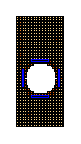
\includegraphics[width=0.32\columnwidth]{icra2018/ip_density_cc_2}
	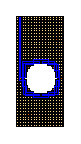
\includegraphics[width=0.32\columnwidth]{icra2018/ip_density_cc_4}
	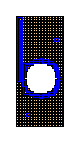
\includegraphics[width=0.32\columnwidth]{icra2018/ip_density_cc_8}
	\caption{Optimal cycle covers with different density scaling. The middle has twice and the right instance has four times the density as the left. {In these instances, the cost of a $90^\circ$ is five times that of a straight pixel transition.}}
	\label{fig:ip:differentdensities}
	%TODO: this picture can be removed if the paper is too long.
	\vspace{-1em}
\end{figure}

\paragraph{Tours}
Computing a minimum cycle cover may result in several subcycles that need to be visited separately, which is appropriate
for the use of several UAVs or when several separate roundtrips by the same UAV are convenient.
If we want to determine connected roundtrips by a single UAV, we need to connect the components of
a cycle cover to a tour. This can be achieved via integer programming by adding additional constraints for
separating these {\em subtours}.

%Separation constraints
This separation of subtours is more complicated than for the classic TSP because there may be tours that 
cross but are not connected. Instead of connecting two subtours, one subtour can also be discarded.

% Second constraint is sufficient but inefficient because it cannot efficiently force to distant subtours to connect.
We first consider a constraint (Eq.~\ref{eq:gg:fc:ip1:subcycle:2}) that is able to separate any given solution with multiple subtours.
Let $Q$ be the pixels of a selected subtour. 
Let $p_\ell\in Q$ be a pixel with high density and no other subtours crossing it
%(if this is not possible, one can assume the subtours covering this field to be
%connected), 
and $p_{\ell'}\not\in Q$ be another covered pixel with high density.
These two pixels are used for `defusing': if one of them is no longer covered, the constraint is automatically fulfilled.
We denote by $Q_s$ the pixels that are covered only by straight paths in the subtour.
%We denote by $Q_s$ the pixels that are covered only straight by the subtour.
$T(p_j)$ describes the turn variables of a pixel $p_j$.
$x'$ refers to the variable assignment in the current solution.
%\begin{strip}
%\begin{equation}
%	y_{\ell}+y_{\ell'}+\sum_{p_i,p_k\in N(p_\ell), x'_{i\ell k}=0} x_{i\ell k} + \sum_{t\in T(v), v\in Q_s-p_\ell} t + \sum_{ p_j\in Q\setminus (Q_s+p_\ell), p_i\not=p_k\in N(p_j), x'_{ijk}=0} x_{ijk} \geq 1 \label{eq:gg:fc:ip1:subcycle:2}
%\end{equation}
%\end{strip}
\begin{align}
	1 \leq y_{\ell} &+y_{\ell'}+\sum_{p_i,p_k\in N(p_\ell), x'_{i\ell k}=0} x_{i\ell k}  + \sum_{t\in T(v), v\in Q_s-p_\ell} t \nonumber \\
	   & + \sum_{ p_j\in Q\setminus (Q_s+p_\ell), p_i\not=p_k\in N(p_j), x'_{ijk}=0} x_{ijk} \label{eq:gg:fc:ip1:subcycle:2}
\end{align}


While this constraint suffices for capturing the mathematical conditions, its practical performance is unsatisfactory
for connecting distant subtours. A better approach is described in the following;
this is not always sufficient but more efficient in connecting distant cycles. 
We use the same definitions as for the previous constraint, but consider an additional set $Q'$ that is a superset of $Q$.
$Q$ are the pixels of a subtour and $p_{\ell}$ is a valuable pixel. $Q'$ is a superset of $Q$ (possibly equal to $Q$). $p_{\ell'}$ is a valuable
pixel outside of $Q'$. 
The constraint enforces that either $p_{\ell}$ or $p_{\ell'}$ is uncovered, or there is a path on 
the margin of $Q'$ that connects $p_{\ell}$ and $p_{\ell'}$.

\begin{equation}
	\displaystyle y_{\ell}+y_{\ell'}+\sum\limits_{x\in \text{Leaving}(Q')} x \geq 1
\end{equation}
We use two ways to choose $Q'$ for 
%each of the different 
{these} subtour elimination constraints:
	$Q'=Q$ which is similar to the classical TSP constraint or 
	%\item $Q'$ a sliced of part of the environment (horizontal or vertical cut through the environment). %Not implemented in new implementation.
	$Q'$ is the Voronoi cell of the subtour. %Voronoi cells of close subtours are merged. %Not in the new implementation but I think this was a good idea. Possibly reimplement it.

\subsection{Computational Results}
\label{subsec:computational}

\begin{figure}[h]
	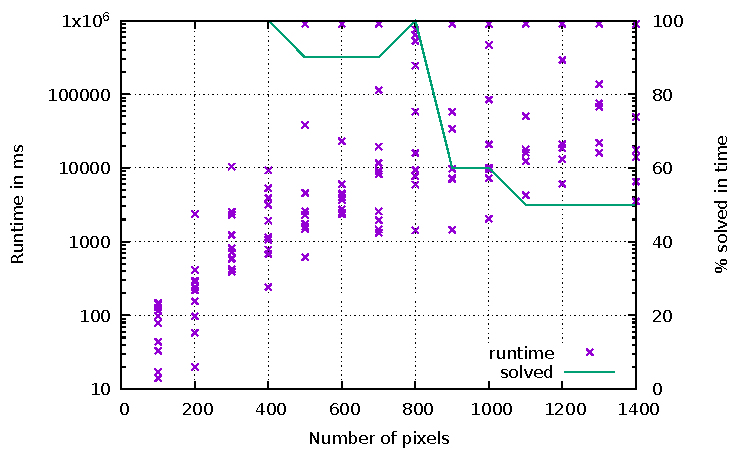
\includegraphics[width=\columnwidth]{icra2018/runtime_cc_optimal_random.pdf}
	\caption{Runtime of solving benchmark instances to optimality. Shown
	are the times of ten instances for each size, with a timeout at \SI{900}{\second}, as
well as the percentage of solved instances. Only the number of turns is minimized in these instances.} \label{fig:experimentsfromthesis}
\vspace{-1em}
\end{figure}

We evaluated the effectiveness of our optimization method by testing it on a suite of benchmark instances based on
random natural grid graphs with random densities; %corresponding to the setting of mosquito distributions,
the probability of a pixel to be added during test instance generation is correlated with its neighborhood, resulting in smoother boundaries which are more natural than purely random instances.
% Changed the sentence above. It didn't make any sense to me.
The tests were carried out for \num{10} instances for each size in the range up to \num{1400} pixels. 
We used modern desktop computers equipped with an \emph{Intel(R) 
Core(TM) i7-6700K CPU @ \SI{4.00}{\giga\Hz}} and \SI{64}{\giga\byte} of RAM. The integer programs were computed with CPLEX version 12.5.0.0 
and the parameters \texttt{EpInt=0}, \texttt{ EpGap=0}, \texttt{ EpOpt=1e-9}, and \texttt{ EpAGap=0}.
Fig.~\ref{fig:experimentsfromthesis} shows runtimes for solving penalty cycle cover to optimality. 
Instances that took longer than \SI{15}{\minute} were aborted.
As shown in the figure, 
even at \num{1400} pixels we were still able to solve half of the instances to provable optimality.
Even for the aborted instances, the computed solutions were within a few percentage points of
the provable lower bound, meaning that they were nearly optimal.

%PC stats, copied from thesis.

Fig.~\ref{fig:ipexample} shows an example of iteratively computing an optimal tour with the described integer program.
This example took less than a minute of total computing time.
It assumed that $90^\circ$ turns cost five times as much as a straight pixel transition (distance).
%but other instances are much more problematic. %such that selecting and connecting a subset of cycles instead of separating the integer program is more practical.

\begin{figure}
	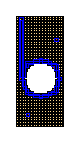
\includegraphics[width=0.24\columnwidth]{icra2018/ip_density}
	
\includegraphics[width=0.24\columnwidth]{icra2018/ip_density_r_1}
	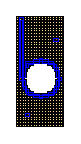
\includegraphics[width=0.24\columnwidth]{icra2018/ip_density_r_2}
	
\includegraphics[width=0.24\columnwidth]{icra2018/ip_density_r_3}
	\caption{Left is an optimal penalty cycle cover. Cycles (blue) cover all areas with high density. After three applications of the tour constraints, a single cycle remains (right). In the intermediate solutions, the subcycles first try to evade the new constraints by reshaping. The final tour omits two of the small hotspots because the cost of integrating them into the single 
tour is prohibitively expensive.}
\vspace{-1em}
	\label{fig:ipexample}
\end{figure}
